
\chapter{Literature Review}
\label{chap:2}
In this chapter, study on related works including clarifications for the main terms utilized in this theory has been discussed. As well analysis of related study on this field has been referenced here. 

\section{Analysis of Related Work}
Now a days researchers has a great interest in management of NDD. But there are lack of effective  research work in this topic. Mainly four types of NDD attract the researchers most. They are Alzheimer’s, Dementia, Parkinson and Schizophrenia. Because they are most occurred disease among the elder people.
That's why patients of these disease are most common in our hospital. To improve their condition researchers from all over the world are working to make their condition better using current technology which include IoT and Machine Learning.
 According to the google scholar, from 2014 to 2020 there are total 164 research paper has been submitted to google scholar which is shown in fig  \ref{fig:chart1}
 \begin{figure}[ht]
   \centering
   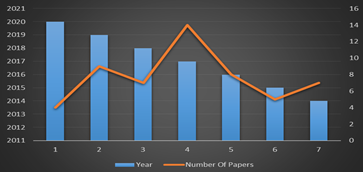
\includegraphics[width=5.5in]{Chap2/chart1.png}
   \caption{Bar Chart of published papers of NDDs where both ML and IoT has been implemented }
   \label{fig:chart1}
\end{figure}
 where ML and IoT both has been implemented. We can clearly depicted from the graph that the curve of research work is increasing day by day. In 2014 there were only 4 related papers in google scholar which was NDD based. But in 2020 the number of related paper has increased to 14 which reflect that, Researchers are getting more interested in this field day by day. 
 Figure \ref{fig:chart2} shows the  percentage of using ML for these four NDD diseases. We can see that the most researched NDD disease is Dementia. Among the elderly people these kind of patients is also increasing day by day. There is no appropriate medicine for these disease. That's why researcher are working to make their life better with the help of IoT and Machine Learning. After Dementia Schizophrenia is the second largest NDD which attract the researchers most. Now a days, Alzheimer's and Parkinson also attract the new researcher.  
 %\ref{fig:chart2}
 \begin{figure}[ht]
   \centering
   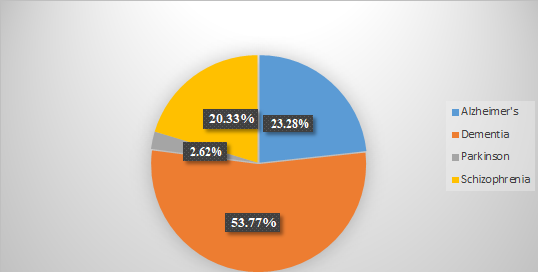
\includegraphics[width=5.5in]{Chap2/chart2.png}
   \caption{Pie Chart of research works regarding ML Approaches in the detection of NDDs }
   \label{fig:chart2}
\end{figure}Therefore researchers also have shown us some work in these field using IoT. Figure \ref{fig:chart3}
%\ref{fig:chart3}
 \begin{figure}[ht]
   \centering
   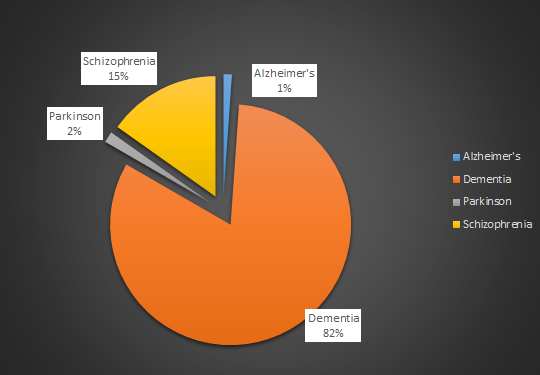
\includegraphics[width=5.5in]{Chap2/chart3.png}
   \caption{Pie Chart of related works with IoT Approaches in detection of NDDs}
   \label{fig:chart3}
\end{figure}describes the percentage of only IoT works in these field for four main NDD diseases. But it is more effective if we can use both ML and IoT in the management of NDD. For the dementia patients 80\% of total  researches are done using both ML and IoT which is shown in fig \ref{fig:chart4}
%\ref{fig:chart4}
 \begin{figure}[ht]
   \centering
   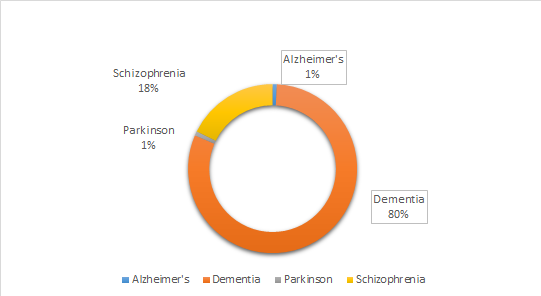
\includegraphics[width=5.5in]{Chap2/chart4.png}
   \caption{Pie chart of research works regarding ML and IoT approaches in the detection of NDDs}
   \label{fig:chart4}
\end{figure}


\section{Related Research Works}
This segment portrays the related works in the management of NDD. We have showed related works on Fall Detection, Wearable device based NDD, Machine Learning based NDD management, IoT based NDD management, Cloud framework based NDD management, Cloud Security, Voice signal based management and Facial expression based NDD management.  
For the reviews of related work we have used the following parameters and notations.\\
Parameters- 1:Architecture, 2:Applications, 3:Open Issues and Challenges, 4:Taxonomy, 5:Security\\

\vspace{0.15cm}
Notations- \checkmark: Considered, and \textit{\sffamily X}: Not Considered




\subsection{Related Works on Fall Detection in management of NDD}
Fall is esteemed to be one of the basic issues for the old patient having neurological issues as it might cause injury or demise. Falls are the main source of incidental passing and the seventh driving reason for death in individuals matured 65 or over having neurological problems. Every year an expected 646 000 people to die from falls internationally of which more than 80\% are in low-and average paid countries. Researchers tried to detect fall remotely with the help of Machine Learning technique. If fall event can be detected more accurately then care giver does not need to be present with the patient all the time. With the help of Smart Home Researches also tried to make their current state better if there occurs a fall event. Researchers have tried to make a system where Message will be automatically send to the caregiver and family member if there occurs a fall event.

\vspace{0.5cm}
Table \ref{tab:fall} shows related works on Fall Detection.
\begin{table}%[ht!]
    \centering
     \caption{Related research works on Fall Detection}
     \vspace{2pt}
  
     \begin{tabular}{|p{1.5cm}|p{0.8cm}|p{3.2cm}|p{3.2cm}|p{2cm}|p{0.17cm}|p{0.17cm}|p{0.17cm}|p{0.17cm}|p{0.17cm}|}
    \hline
  
   \textbf{Author}&\textbf{Year}&\textbf{Objectives}&\textbf{merits}&\textbf{Demerits}&\textbf{1}&\textbf{2}&\textbf{3}&\textbf{4}&\textbf{5}\\\hline
   
   Sase et al. \cite{sase_human_2018}&2018&Introduced a method for detecting fall using depth videos.&ROI is calculated which helps to detect fall by comparing it to calculated threshold.&Doesn’t applicable if the person lying on the floor.&\checkmark&\textit{\sffamily X}&\checkmark&\textit{\sffamily X}&\textit{\sffamily X}\\\hline
   Mostarac et al.\cite{mostarac_system_2011}&2018&Narrated a system that can detect fall with the use of three axis accelerametric data. %including ZigBee transceiver
&Low power consumption, portability, and small size.%the ability to be
%mounted in small pockets %inside the clothes of patients
&Lack discussions about the post fall condition.&\checkmark&\textit{\sffamily X}&\checkmark&\textit{\sffamily X}&\checkmark\\\hline

Doulamis et al.\cite{doulamis_real-time_2010}&2010&Offered a system detecting falls which uses the background subtraction approach. %using hierarchical motion estimation and Gaussian Mixtures which is not sensitive to camera movement
&Uses a single camera with low resolution and low cost.&Discussion of privacy is not covered properly.&\checkmark&\checkmark&\checkmark&\textit{\sffamily X}&\textit{\sffamily X}\\\hline

Ali et al. \cite{ali_using_2018}&2018&Proposed a quick and precised framework to distinguish falls by recordings caught by observation cameras. %on the basis of spatial based features using adaboost and j48 classifier.
&Provide better performance to differentiate between the process of sit and fall.% compared to existing algorithms
&Less efficient in multiple people environment.&\checkmark&\checkmark&\checkmark&\checkmark&\checkmark\\\hline

Bhandari et al.\cite{noauthor_novel_nodate}&2017&Proposed a strategy to identify fall by utilizing the Shi-Tomasi algorithm which is followed by the Pyramidal Lucas-Kanade algorithm. %to process the videos %which simply finds interest points from video frames and computes optical flow to estimate speed of motion.
&This method does not call for any complicated processing of videos and %based on vison based approach which
reduces discomfort caused by wearable devices&The method is applicable only for UR fall detection dataset.&\checkmark&\checkmark&\textit{\sffamily X}&\checkmark&\textit{\sffamily X}\\\hline
Theodo-ridis et al. \cite{theodoridis_human_2018}&2018&Introduced a method to detect fall based on Recurrent Neural Network. %using data acquired from a body-worn accelerometer.
&Can identify falls without false positive detection keeping the total system low cost. %and having a wide spatial area where the approach can be implemented
&Lack discussion about camera data.&\checkmark&\textit{\sffamily X}&\checkmark&\textit{\sffamily X}&\checkmark\\\hline

Kepski et al. \cite{kwolek_human_2014}&2015&Proposed an architecture which can detect fall with camera depth videos.
&Acquire real-time data and detect all types of fall with low cost.&No discussion about data security.&\checkmark&\textit{\sffamily X}&\checkmark&\textit{\sffamily X}&\textit{\sffamily X}\\\hline
       
    \end{tabular}
    \label{tab:fall}
\end{table}

\subsection{Related research works on Applications of wearable devices in management of NDD}
NDD management can be done by both vision based and non vision based sensors. Vision based sensors are depth camera, kinect camera by Microsoft etc. Non vision based sensor are implemented on the wearable device. There are mainly two non vision based wearable sensors to manage elderly patients. They are accelerometer and gyroscope. Fusion of these two sensors give better accuracy performance than using a single sensor. Researchers are now trying to fused both accelerometer and gyroscope in their work. They are also integrating wireless network with these sensor to collect data remotely. 

\vspace{0.5cm}
Table \ref{tab:wearable device} shows related works of wearable device with wireless network technology in management of NDD.
\begin{table}%[ht!]
    \centering
     \caption{Related research papers on wearable device with wireless network technology in management of NDD}
     \vspace{2pt}
  
    \begin{tabular}{|p{1.5cm}|p{0.8cm}|p{3.2cm}|p{3.2cm}|p{2cm}|p{0.17cm}|p{0.17cm}|p{0.17cm}|p{0.17cm}|p{0.17cm}|}
    \hline
  
   \textbf{Author}&\textbf{Year}&\textbf{Objectives}&\textbf{merits}&\textbf{Demerits}&\textbf{1}&\textbf{2}&\textbf{3}&\textbf{4}&\textbf{5}\\\hline
Pierleoni et. al. \cite{noauthor_high_nodate}
&2018
&Proposed a system to detect fall using magnetometer, gyroscope and accelerometre. %with efficient data
%fusion and fall detection algorithms
&Overcome the limitation of a single accelerometer %by using MARG (Magnetic, Angular Rate,
%and Gravity) sensors.
&Data security is not discusses properly&\checkmark&\checkmark&\checkmark&\checkmark&\textit{\sffamily X}\\\hline


Baga et al. \cite{baga_perform_2009}
&2009
&Offer a system that can %monitor and 
manage neurodegenerative by minimzing the wearable sensors %for daily patients
&presented a
modular system architecture that can be adapted to any disease
&Lack discussion of the detection and quantification% algorithm into
%the wearable device
&\checkmark&\textit{\sffamily X}&\checkmark&\checkmark&\checkmark\\\hline

Avvenuti et al. \cite{noauthor_wireless_nodate}
&2010
&Proposed a monitoring system where sensors collect real-time data %from patient and
also process before send alert to the caregiver. %Patient’s information then send to the nurse care station further process via a gateway server.
&Can collect data both wearable and wirelessly and and sends alert to caregiver %if there need any help in the time of emergency it sends an alert to the caregiver. Patient can be monitored all day long.
&More bandwidth needed.
&\checkmark&\textit{\sffamily X}&\checkmark&\checkmark&\textit{\sffamily X}\\\hline
 
 Wang et al. \cite{wang_wifall_2017}
&2016
&Proposed a device free fall detection model 'Wifall' with the help of wireless network.
&Can work without hardware modification,extra environmental setup %or any wearable device
&Efficient only for single people environment.
&\checkmark&\textit{\sffamily X}&\checkmark&\checkmark&\textit{\sffamily X}\\\hline
LeMoyne et al.\cite{lemoyne_implementation_2015}
&2015
&Intends to join a Smartphone as a stage for remote accelerometers Machine learning %to identify deep brain characteristics Stimulator on and off status for the ultimate tremor
&integrate three mature systems deep brain stimulation, a smartphone and ML successfully    %\textbf{Author}&\textbf{Year}&\textbf{Objectives}&\textbf{merits}&\textbf{Demerits}&\textbf{1}&\textbf{2}&\textbf{3}&\textbf{4}&\textbf{5}\\\hline

 % to improve the efficiency of deep brain stimulation treatment
&Need developments in
miniaturization
&\checkmark&\textit{\sffamily X}&\checkmark&\checkmark&\textit{\sffamily X}\\\hline
Busta-mante et al. \cite{noauthor_wireless_nodate2}
&2008
&Proposed an Personal Remote Monitoring Device %which collects data from patients with different sensors and send it to the hospital computer via a 
with RF radio transceiver.
&different layers of software and hardware architecture can work independently.% One layer's failure will not affect another.
&used only for the PD and Alzheimer's patients %due to some lack of sensor establishment. Different sensors used here must be carried with patients all over body.
&\checkmark&\checkmark&\checkmark&\textit{\sffamily X}&\textit{\sffamily X}\\\hline
Tisch et al. \cite{noauthor_detection_nodate}
&2012
&Distinguish Alzeimer and PD by nanomaterial sensors and Breath test.
&%As both diseases are quite similar but the treatment of these diseases have some non-similarities and the research 
can identify the some non-similaritiesbetween both disease effectively.
&They can only detect, can not manage it.
 
 &\textit{\sffamily X}&\textit{\sffamily X}&\checkmark&\checkmark&\textit{\sffamily X}\\\hline
 \end{tabular}
    \label{tab:wearable device}
    \end{table}

\subsection{Related research works on Applications of ML in management of NDD}
Machine Learning approach provide a great interest to the researcher in the management of NDD. In the machine learning process, a learning algorithm trains different forms of fall and daily living activity (ADL)
patterns, and then an occurrence is labeled as a fall or ADL by adding it to an estimation algorithm.
The machine learning approach is more advanced and results
in better detection rates of more than 95\% accuracy. Unfortunately, because of the high computing and capital needs,
it is hard to apply the machine learning approach.


 
\vspace{0.5cm}
Table \ref{tab:DL} shows related works of ML approaches in management of NDD.
\begin{table}%[ht!]
    \centering
     \caption{Related research works on ML approaches in management of NDD }
     \vspace{2pt}
  
     \begin{tabular}{|p{1.5cm}|p{0.8cm}|p{3.2cm}|p{3.2cm}|p{2cm}|p{0.17cm}|p{0.17cm}|p{0.17cm}|p{0.17cm}|p{0.17cm}|}
    \hline
  
   \textbf{Author}&\textbf{Year}&\textbf{Objectives}&\textbf{merits}&\textbf{Demerits}&\textbf{1}&\textbf{2}&\textbf{3}&\textbf{4}&\textbf{5}\\\hline

Zebin et Al.\cite{zebin_human_2016}	&2016	&Presented a feature learning system to automate feature gaining from crude contributions for movement acknowledgment using CNN.	&Classification accuracy is high contrasted with SVM and MLP	&Other application of activity recognition is missing.
 &\checkmark&\textit{\sffamily X}&\checkmark&\textit{\sffamily X}&\textit{\sffamily X}\\\hline

Hossain et Al. \cite{hossain_audio-visual_2019}	&2018	&A general media feeling acknowledgment framework was proposed via DL approach	&Can be integrated in any emotion-aware intelligent systems
which increases  the effectiveness	&Focused on application not the open issues.
 &\textit{\sffamily X}&\checkmark&\textit{\sffamily X}&\checkmark&\textit{\sffamily X}\\\hline
Ravi et Al.\cite{ravi_deep_2017}	&2017	&Proposed a deep learning methodology which combines feature learning with correlative data from a bunch of shallow highlights.&Provide better performance than current state-of-the-art approaches by real time on-node computation.	&Lack discussion about cost effectiveness.

&\checkmark&\textit{\sffamily X}&\checkmark&\textit{\sffamily X}&\checkmark\\\hline
  \end{tabular}
    \label{tab:DL}
    
\end{table}

\subsection{Related papers on Applications of IoT in management of NDD}

 IoT devices are now frequently being used in management of NDD. Through IoT patients can be monitored remotely without being present there physically such as turn the light, fan switch on off. Researcher are trying hard to make a NDD patient current state better with the help of IoT because there are no successful treatment for these diseases and patient need to stay in the home. It is also not possible to stay beside the patient all the time. So IoT can help us to manage these kind of patient in their own home without presence of the doctor and caregiver.
\vspace{0.5cm}
Table \ref{tab:IOT} shows related works on Applications of IoT in management of NDD.
\begin{table}%[ht!]
    \centering
     \caption{Related works on Applications of IoT in management of NDD}
     \vspace{2pt}
  
     \begin{tabular}{|p{1.5cm}|p{0.8cm}|p{3.2cm}|p{3.2cm}|p{2cm}|p{0.17cm}|p{0.17cm}|p{0.17cm}|p{0.17cm}|p{0.17cm}|}
    \hline
  
   \textbf{Author}&\textbf{Year}&\textbf{Objectives}&\textbf{merits}&\textbf{Demerits}&\textbf{1}&\textbf{2}&\textbf{3}&\textbf{4}&\textbf{5}\\\hline
Gia et al. \cite{nguyen_gia_energy_2018}
&2018
&Introduced an IoT-based wearable system to to ensure a appropriate
degree of control and reliability of a fall detection system.
%This method tried to discusse the most appropriate solution in terms of energy
&Efficiency, feasibility, and complexity where the wearable nodes are low-cost,lightweight and flexible.
&Short operating
duration, discontinuation of services or unreliability.&\checkmark&\textit{\sffamily X}&\checkmark&\textit{\sffamily X}&\textit{\sffamily X}\\\hline

Chatter-jee et. al \cite{chatterjee_iot-based_2017}
&2017
&Proposed an intelligent healthcare system with the help of IoT and Decision Support System. %to empower the physicians %with increased level of insights into patients’ data.
&Low cost, ambient
assisted living and improved
experience for patients.
&Lack discussion on uses in healthcare environments.
&\checkmark&\textit{\sffamily X}&\checkmark&\checkmark&\textit{\sffamily X}\\\hline

Tzallas et al.\cite{tzallas_perform_2014}
&2014
&Introduced a system named PERFORM for the real-times remote observation, evolution and management of PD
&Provide a simple, safe,
painless and non-invasive assistance to the clinician neurologist %to determine the optimal
%therapeutically schema.
&Privacy of patient’s data are not declared properly.
&\checkmark&\checkmark&\checkmark&\textit{\sffamily X}&\textit{\sffamily X}\\\hline

Pereira et al. \cite{noauthor_mobile_nodate}
&2000&Has built up a portable mobile application for the help of individuals of PD patients.
&Provide knowledge and professional upholding both patients and caregivers. %to improve healthcare assistance
&Lack of discussion about feedback management. %and maintainance of the application.
&\textit{\sffamily X}&\checkmark&\checkmark&\textit{\sffamily X}&\checkmark\\\hline
Wankhe-de et al.\cite{wankhede_aid_2019}
&2019
&Discusses the action of the pupil Sensor monitoring and head motion network attached to an IoT Infrastructure. %to improve ALS patient's everyday function
&ALS patient with this system will be free enough to handle equipment and to control the door safety.%so there's not much need for the caregiver to do that 24/7
&Focus on devices not the open issues.
&\checkmark&\checkmark&\textit{\sffamily X}&\textit{\sffamily X}&\textit{\sffamily X}\\\hline

Punin et Al. \cite{punin_wireless_2017}
&2017
&Created non-intrusive equipment based remote framework with FOG to gather information from PD patients. %with FOG to induce progress of walking, avoid falling, and enhance the lifestyles of patients.
&Small body weight,
ergonomic and open to people with limited resources.
&Cost effectiveness is low. %as the system need at least medium level processor.
&\checkmark&\checkmark&\textit{\sffamily X}&\textit{\sffamily X}&\checkmark\\\hline

    \end{tabular}
    \label{tab:IOT}
    
\end{table}



\subsection{Related works on Cloud based framework for the patient management suffering from NDD}
Medical data are now being stored and processed in the cloud and it is becoming popular day by day as the patient can get the instructions from the doctor without their physical appearance. Cloud based framework also reduce the cost of patient management as caregiver does not to be present there all the time. Smart Home integrating with cloud also provide better result in the management of NDD. But the researcher face the problem most in the cloud based management is security as hacker can easily hack to the cloud and can get accent to sensitive information.
Table \ref{tab:cloud} shows related papers on Cloud based framework for the management of NDD.
\begin{table}%[ht!]
    \centering
     \caption{Related works on Cloud Based framework for the patient management suffering from NDD }
     \vspace{2pt}
  
    \begin{tabular}{|p{1.5cm}|p{0.8cm}|p{3.2cm}|p{3.2cm}|p{2cm}|p{0.17cm}|p{0.17cm}|p{0.17cm}|p{0.17cm}|p{0.17cm}|}
    \hline
    

  
   \textbf{Author}&\textbf{Year}&\textbf{Objectives}&\textbf{merits}&\textbf{Demerits}&\textbf{1}&\textbf{2}&\textbf{3}&\textbf{4}&\textbf{5}\\\hline
   
  Al Mamun et al. \cite{noauthor_cloud_nodate}
&2015
&Proposed a cloud based framework for patients from rural area getting instructions from doctors by sending voice recording to the cloud manager %via internet.
&PD can be detected and diagnosis very easily only with patient’s voice samples. %where they need a smartphone with internet connection.
&The framework only detect PD by voice.&\checkmark&\textit{\sffamily X}&\checkmark&\textit{\sffamily X}&\textit{\sffamily X}\\\hline
   
Pan et al. \cite{noauthor_jmu_nodate}
&2015 &Suggested a model "PD Dr" mobile cloud-based mHealth application. %that would collect analytical and empirical PD information for home-based management and analysis of significant of symptoms that used a 3D smartphone accelerameter and transmit information 
&PD Dr tests hand-resting shake, walk and turn. %that have a good combination of motor performance with PD intensity. 
&Can not provide long-term continual assessment. %and based on only tremor and gait evaluation in PD.
&\checkmark&\checkmark&\textit{\sffamily X}&\textit{\sffamily X}&\textit{\sffamily X}\\\hline

Al Hussein et al. \cite{alhussein_monitoring_2017}
&2017
&Proposed a framework to transmit voice signal to cloud and processed the signal to detect PD. %and send it to the registered doctor who give the necessary instructions to the patient via cloud.
&Two different database and four ML classifiers are used where the accuracy level is upto 97\%.
&Not applied in real-life atmosphere. %and its only collect voice data not the other symptoms of the PD.
&\checkmark&\checkmark&\textit{\sffamily X}&\textit{\sffamily X}&\textit{\sffamily X}\\\hline

Depari et al. \cite{depari_iot_2019}
&
2019&
Proposed an architectural model to connect prototype instruments to the cloud. %which gives a secure real-time interaction with the developers and the operators. 
&Offers low-cost real-time data, stable, accessible and compatible message-oriented strategies. %and enables info from additional sensors that involved.
&Can not be used for interchanging raw and meta data. %and that’s why the MCPS interface is missing.
&\checkmark&\textit{\sffamily X}&\checkmark&\textit{\sffamily X}&\checkmark\\\hline
Ivan et al. \cite{noauthor_fog_nodate}&
2019
&Proposed an application which collects image data and 3D scenes transmitting in cloud. %only when it integrate to saves the network traffic and bandwidth.
&Only sends final evolution result to cloud which saves bandwidth also make the network fluffy.
&Collects certain information only.
&\checkmark&\checkmark&\checkmark&\textit{\sffamily X}&\textit{\sffamily X}\\\hline

Akhund et al. \cite{niamat_ullah_akhund_adeptness_2018}
&2018
&Proposed a wearable device for Alzeimer’s patients that collects different data from patients and send it to cloud. %database where the data is processed to tell the condition of patient
&By using various sensors it can give a feasible result and the accuracy level is quite acceptable. %It notify all the time to the caregiver about the patient.
&It can just notify or detect the diseases, not manage it.
&\checkmark&\textit{\sffamily X}&\checkmark&\textit{\sffamily X}&\textit{\sffamily X}\\\hline
   
   \end{tabular}
    \label{tab:cloud}
\end{table}






\subsection{Related papers on cloud security in management of NDD}

 
As cloud based framework is becoming popular in the management of NDD so cloud based security is a prime concern for the developers in this field. To secure sensitive information from the unwanted person researchers are also working hard in these field now days. 
Table \ref{tab:security} shows related works of Cloud Security in management of NDD.
\begin{table}%[ht!]
    \centering
     \caption{Related works of Cloud Security in management of NDD}
     \vspace{2pt}
  
    \begin{tabular}{|p{1.5cm}|p{0.8cm}|p{3.2cm}|p{3.2cm}|p{2cm}|p{0.17cm}|p{0.17cm}|p{0.17cm}|p{0.17cm}|p{0.17cm}|}
    \hline
  
   \textbf{Author}&\textbf{Year}&\textbf{Objectives}&\textbf{merits}&\textbf{Demerits}&\textbf{1}&\textbf{2}&\textbf{3}&\textbf{4}&\textbf{5}\\\hline
Khan et al.\cite{noauthor_cloud-based_nodate}	&2014	&Proposed a secure architecture with wireless body area networks (WBANs) where sensor communicate with bio-metric key.	&Data communication maintain privacy and security generating multiple bio-metric key	&Quite expensive to use.
&\checkmark&\textit{\sffamily X}&\checkmark &\checkmark&\checkmark\\\hline

Chen et al. \cite{chen_privacy_2016}	&2016	&Proposed a cloud based system which is flexible with a wearable device of encrypt method.	&Users are divided along their data with adequate security and prevent malicious attacks.	&One-way process. Can’t give instruction to the patient.
&\checkmark&\checkmark&\checkmark &\checkmark&\checkmark\\\hline

Hamid et al. \cite{noauthor_security_nodate}	&2017	&To Suggest private health details safely in the cloud using a fog storage facility.	&Encryption process can create a symmetric key	&One can not communicate with others in the time of emergency.
&\checkmark&\textit{\sffamily X}&\checkmark &\checkmark&\checkmark\\\hline

Lohr et al. \cite{lohr_securing_2010}	&2010	&Suggested a framework for giving the appropriate security to the client’s infrastructure.	&Merge both the security of client and network.	&Can not solve usability problems in daily life.
&\checkmark&\textit{\sffamily X}&\checkmark &\checkmark&\checkmark\\\hline

\end{tabular}
    \label{tab:security}
    
\end{table}

\subsection{Related papers on integration of voice signal in management of NDD}

 
Because of low cost management predictive screening strategies for older people having NDD, dependent on voice have attracted prominence. NDD can be also detected using the voice signal of the patients. Doctor can detect NDD remotely with the help of NDD. Besides NDD management can also be done with voice signal. In the smart home voice control system can also be implemented to manage NDD diseases. Researcher have shown a lot of possibilities in these field to make a better life for NDD patient. 

Table \ref{tab:audio} shows related works on integration of audio signal in management of NDD.
\begin{table}%[ht!]
    \centering
     \caption{Related papers on integration of voice signal in the management of NDD}
     \vspace{2pt}
  
     \begin{tabular}{|p{1.5cm}|p{0.8cm}|p{3.2cm}|p{3.2cm}|p{2cm}|p{0.17cm}|p{0.17cm}|p{0.17cm}|p{0.17cm}|p{0.17cm}|}
    \hline
    \textbf{Author}&\textbf{Year}&\textbf{Objectives}&\textbf{merits}&\textbf{Demerits}&\textbf{1}&\textbf{2}&\textbf{3}&\textbf{4}&\textbf{5}\\\hline
    
    Doukas et al. \cite{doukas_advanced_2008}	&2008	&Proposed an architecture to detect fall via fall sound and patient’s motion.	&Fall detection is possible with the voice of fall and notify in the time of emergency.	&Carrying sensors in the body.
    &\checkmark&\textit{\sffamily X}&\checkmark &\textit{\sffamily X}&\checkmark\\\hline
    
    
M. Pham et al. \cite{minh_pham_cloud-based_2016}	&2016	&To proposed a smart home plan to monitor patient’s activity and give a proper report to the caregiver.	&The perfect home setup helps to collect appropriate data for processing.	&Will not provide any help in the term of emergency.
 &\checkmark&\textit{\sffamily X}&\textit{\sffamily X}&\checkmark &\checkmark\\\hline
E. Principi et al.\cite{principi_integrated_2015}	&2015	&To suggest an architecture for integrating audio signal in the time of emergency.	&Send abnormal movement and by delivering voice command home automation will work. 	&Roust voice ratio can not work.
 &\checkmark&\checkmark &\checkmark&\textit{\sffamily X}&\textit{\sffamily X}\\\hline
  
   

\end{tabular}
    \label{tab:audio}
    
\end{table}


\subsection{Related papers on detection of facial expression from video sequences to analyze patient's current state suffering from NDD}

 In detection and recognition of facial expression studies, emotional states are distilled into six facial profiles, comprising pleasure, rage, sadness, disgust, discomfort, and fear, and are also analysed. Achieving automated identification and comprehension of facial emotions will facilitate advancement of applications such as pain and distress recognition, and manipulation identification and distress control in relevant disciplines, such as information systems, communications devices, and medical technology. Facial expression identification has been of considerable importance in science due to the clinical benefit and scientific relevance of clinical and cognitive sciences \cite{pantic_face_2006}.
Advances in legitimate research sub-fields, such as face detection[6], monitoring and recognition[7] and new advances in computational areas, such as automated learning[8, 9] and feature extraction, have recently made substantial progress in this area. However, due to the evolving, nuanced and gradual shifts in facial expression and multiple head movements, exact identification of facial expressions is still a difficult question \cite{rein-lien_hsu_face_2002} \cite{fang_rank-n_2009}.
Most modern techniques of identification of facial expression have focused on means of evaluating the rational appearance frame or optimum step frame of each of the six simple video sequence expressions (i.e. recognition of static-based facial expression) \cite{cornelis_vaguely_2007}. The static approach analyzes facial expressions and dismisses certain essential properties of adaptive expressions. Consequently, in some multilevel thresholding, this mechanism fails miserably. The adaptive approach derives details about time and movement from the image sequence of facial gestures. Evolving traits providing valuable data reflecting underlying psychological state are the rotation of feature points and variations in facial texture. Diverse data can also be collected during facial expression detection from across the whole video series.

 
 Audio and video data are now commonly being used by the researchers to develop a better management system for NDD patients.
 Table \ref{tab:video} shows related works on detection of facial expression from video sequences to analyze patient's current state suffering from NDD.
 \begin{table}%[ht!]
     \centering
      \caption{Related works on detection of facial expression from video sequences to analyze patient's current state}
      \vspace{2pt}
  
     \begin{tabular}{|p{1.5cm}|p{0.8cm}|p{3.2cm}|p{3.2cm}|p{2cm}|p{0.17cm}|p{0.17cm}|p{0.17cm}|p{0.17cm}|p{0.17cm}|}
     \hline
    \textbf{Author}&\textbf{Year}&\textbf{Objectives}&\textbf{merits}&\textbf{Demerits}&\textbf{1}&\textbf{2}&\textbf{3}&\textbf{4}&\textbf{5}\\\hline
    
   Kamarol et al. \cite{kamarol_spatiotemporal_2016}	  &2016	&Propose an appearance-based template to perform facial expression recognition in video streams.
     &Performs several states of the art expression based feature selection methods.	
     &Classification is easy and not checked during complex movement of the brain.
     &\textit{\sffamily X} &\checkmark &\checkmark &\checkmark &\textit{\sffamily X}\\\hline

  Xie et Al. \cite{xie_video-based_2014} &2014	&Provided a tool that uses the histogram sequence of local gabor binary patterns from three orthogonal planes (LGBP-TOPs).
 &Strong and less complicated machine method.
 &Needs to improve accuracy
 Performances.
 &\textit{\sffamily X}&\checkmark&\checkmark&\checkmark&\textit{\sffamily X}\\\hline

 Suja P et Al. \cite{suja_p_dynamic_2015} &2015	&Propose a geometrically focused method to the
 identification of  six specific emotions in video sequences.
 &Improved accuracy with  comparing to complex methods.	
 &Evaluation cannot be determined under real time conditions.
 &\textit{\sffamily X}&\checkmark&\checkmark&\checkmark&\textit{\sffamily X}\\\hline

 Chiran-jeevi  et Al.\cite{chiranjeevi_neutral_2015} &2015 &Propose a method lightweight vs emotional classification engine that serves as a pre-processor to conventional emotion classification approaches.
 &Computational benefit of using the suggested approaces as a pre-processing device	&Under sudden pose variations, CLM fitting may not be accurate.
 &\textit{\sffamily X}&\checkmark&\checkmark&\checkmark&\textit{\sffamily X}\\\hline

 Shojaei-langari et al.\cite{shojaeilangari_robust_2015} &2015	&Propose a method called severe sparse learning, capable of jointly studying a dictionary and a non-linear model of classification.
 &Under challenging scenarios, gives Better performance.
 &Computa-tional cost is high for both feature extraction and classification.
 &\textit{\sffamily X}&\textit{\sffamily X}&\textit{\sffamily X}&\checkmark&\textit{\sffamily X}\\\hline

    
    
     \end{tabular}
     \label{tab:video}
    
 \end{table}

\section{Research Gap}
Most of the framework proposed by the researchers are only wearable device based or camera sensor based. That's why accuracy is low. Combination of both wearable sensors and mobile sensors has not been successfully implemented yet. 
Besides most of the framework are efficient on single people environment only. If there are more than one people the accuracy level decreases. Management is less discussed in most of the work as researchers only tried to detect the anomaly in their models.Besides, data collected from the sensor is processed in cloud. But how the Cloud will be secured, has not described in most of the work. That's why Privacy is the barrier in NDD management which is not mentioned in most of the work. 